\documentclass{article}
\usepackage[T1]{fontenc}
\usepackage[utf8]{inputenc}
\usepackage{ismir}
\usepackage{amsmath,cite}
\usepackage{graphicx}
\usepackage{color}
\usepackage{booktabs}
\usepackage{enumitem}
\usepackage[hidelinks]{hyperref}
\usepackage[none]{hyphenat}

\title{Continuous and Categorical Conditioning for Pitch Control in Audio Generation with EnCodec}

\oneauthor
  {Manuel Castillo Obreg\'on}
  {Universitat Pompeu Fabra\\Barcelona, Spain}

\def\authorname{M. Castillo Obreg\'on}
\newcommand{\projecturl}{\href{https://github.com/manueleco/pitch-conditioning-study}{GitHub repository}}

% Optional:
% \usepackage[bookmarks=false,pdfauthor={\authorname},pdfsubject={\pdfsubject},hidelinks]{hyperref}

\sloppy
\emergencystretch=1em

\begin{document}

\maketitle

\begin{abstract}
This paper compares two ways of representing a pitch control parameter in an audio generator built with EnCodec tokens. The dataset contains short excerpts from the first two bars of \textit{Fur Elise}. Two matched models are trained with the same data, architecture, and training procedure. They differ only in how \texttt{pitch\_shift} is represented, either as a continuous scalar or as a categorical one hot vector. Evaluation combines validation loss with objective pitch tracking, monotonicity checks, interpolation checks, and onset artifact measurements. The results show that decoding settings have a strong effect on controllability. A balanced inference profile gives the fairest shared comparison because both models remain monotonic, while a cooler sampling profile gives the continuous model its strongest interpolation behavior but destabilizes the categorical model. The study therefore suggests that conditioning representation and decoding strategy should be examined together instead of relying on validation loss alone.
\end{abstract}

\section{Introduction}\label{sec:introduction}

The main question in this project is whether a naturally discrete pitch control should be represented as a continuous value or as a categorical one hot variable in a conditioned audio generation system. The comparison is intentionally narrow. Both models share the same dataset, architecture, EnCodec tokens, splits, and training regime. The only controlled change is the representation of \texttt{pitch\_shift}. This places the study within work on neural audio codecs and controllable music generation, where discrete token pipelines such as Jukebox~\cite{dhariwal2020jukebox}, AudioLM~\cite{borsos2023audiolm}, and systems built with EnCodec~\cite{defossez2022high,copet2023simple} have made raw audio generation and control far more practical.

The project is also constrained by a small compute budget and by the use of a melodic source instead of a pure texture. This makes it especially important to focus the comparison on controllability rather than on raw synthesis quality alone.

\section{Related Work}\label{sec:related_work}

Early work such as Jukebox~\cite{dhariwal2020jukebox} showed that music can be modeled in a compressed latent space while still supporting conditioning variables such as artist, genre, and lyrics. AudioLM~\cite{borsos2023audiolm} further established that language modeling over discrete audio tokens can preserve long term structure in generated audio, making token based raw audio generation a viable research direction.

Closer to the present study, EnCodec~\cite{defossez2022high} provides the neural audio codec used to obtain compact discrete representations with good reconstruction quality. MusicGen~\cite{copet2023simple} demonstrated that EnCodec token streams can support controllable music generation through text and melody conditioning. The current project is narrower than these systems: it isolates one musically meaningful control variable, pitch shift, and compares two representations of that variable while holding data, architecture, and training regime constant.

\section{Why This Question Matters}\label{sec:why_it_matters}

This question is relevant to MIR because stable direct control can be used to generate counterfactual audio examples for probing system behavior. If a pitch controlled generator reacts predictably, it can help create targeted augmentations and controlled probes for tasks such as melody extraction, key estimation, pitch aware retrieval, and transcription. In that sense, the study is enabling rather than only descriptive.

The question is also interesting for music technology beyond MIR research. A reliable conditioning interface is useful for creative coding, music production tools, interactive educational software, and rapid prototyping of controllable audio plugins. The problem is hard because pitch in raw audio is entangled with onset shape, timbre, and the decoding policy itself. The problem is also moderately novel in this exact setup, because the experiment isolates conditioning representation inside a pipeline built with EnCodec instead of changing several architectural factors at once.

\section{Method}\label{sec:method}

\subsection{Dataset}\label{subsec:dataset}

The dataset is built from original performances of the first two bars of \textit{Fur Elise}, recorded in Logic Pro in a home studio. Four intentionally bad source files were excluded. Each retained take was cropped to a short window of approximately \texttt{1.9\,s} and expanded to five pitch levels: \texttt{\{-1.0, -0.5, 0.0, 0.5, 1.0\}} semitones. The final train, validation, and test partitions contain 30 base takes in total, balanced across the five pitch levels, for approximately \texttt{4.75} minutes of audio.

\subsection{Conditioning Variants}\label{subsec:conditioning_variants}

\begin{itemize}[leftmargin=*]
  \item \textbf{Continuous.} \texttt{pitch\_shift} is represented as a scalar value in semitones.
  \item \textbf{Categorical.} \texttt{pitch\_shift} is discretized to fixed classes and expanded to a one hot representation.
\end{itemize}

\subsection{Training and Inference}\label{subsec:training_and_inference}

Both models were trained from the same EnCodec token pipeline and compared primarily through their long runs with early stopping. A later fine tuning stage with a lower learning rate is retained only as an auxiliary observation. During offline generation, state reset and fixed seeds were enforced per sample so that inference settings could be compared fairly. An inference sweep was then run to evaluate how decoding parameters interact with the conditioning representation. The implementation adapts ideas and software components from the official EnCodec and AudioCraft ecosystems~\cite{facebookresearch2022encodec,facebookresearch2023audiocraft}.

\section{Experimental Setup}\label{sec:experimental_setup}

The main evaluation is based on three axes. First, the generated discrete pitch sweep must remain monotonic. Second, the continuous model should ideally interpolate between seen neighbors for \texttt{+0.25} and \texttt{+0.75} semitone requests. Third, the generated audio should avoid strong onset artifacts, which are quantified with onset to body ratios derived from short term spectral measurements.

In addition to training loss, the analysis uses objective metrics extracted from the generated audio: pitch mean absolute error in semitones, pitch stability across voiced frames, monotonicity of the discrete sweep, interpolation consistency, and onset artifact ratios. Pitch tracking is estimated with a YIN procedure~\cite{decheveigne2002yin}, implemented through librosa~\cite{mcfee2015librosa}. This is important because listening alone was not considered sufficient for the final comparison.

\subsection{Companion Code and Reproducibility}\label{subsec:companion_code}

The public companion repository for this project is available as a \projecturl. The main executable narrative is the main notebook in the repository. The repository also includes dedicated scripts for short clip dataset construction, paired conditioning export, model training, inference sweeps, pitch evaluation, and objective audio analysis. A repository level artifact guide summarizes these entry points for readers and reviewers.

\subsection{Visual and Sonic Examples}\label{subsec:visual_and_sonic_examples}

Static figures are stored in \texttt{results/figures/}, and curated listening examples are organized in a listening guide inside the repository. The main shared listening comparison uses the \texttt{balanced\_sample\_1\_9s} profile, while the continuous interpolation showcase uses \texttt{cool\_sample\_1\_9s}. This separation mirrors the quantitative analysis and keeps the sonic examples aligned with the main claim of the study.

\section{Results}\label{sec:results}

\tabref{tab:sweep} summarizes three selected inference profiles. Hereafter, \textit{Baseline} refers to \texttt{baseline\_sample\_3s}, \textit{Cool} refers to \texttt{cool\_sample\_1\_9s}, and \textit{Balanced} refers to \texttt{balanced\_sample\_1\_9s}. Balanced is the main shared reference for the project.

\begin{table}[t]
  \centering
  \scriptsize
  \setlength{\tabcolsep}{3pt}
  \begin{tabular}{llccccc}
    \toprule
    Profile & Model & MAE & Stability & Onset & Mono & Interp. \\
    \midrule
    Baseline & Cont. & 0.216 & 1.235 & 4.444 & yes & no \\
    Baseline & Cat.  & 0.245 & 3.650 & 2.754 & yes & n/a \\
    Cool     & Cont. & 0.131 & 2.148 & 4.581 & yes & yes \\
    Cool     & Cat.  & 1.972 & 3.178 & 2.474 & no  & n/a \\
    Balanced & Cont. & 0.161 & 0.608 & 3.978 & yes & no \\
    Balanced & Cat.  & 0.263 & 4.278 & 2.873 & yes & n/a \\
    \bottomrule
  \end{tabular}
  \caption{Objective metrics for selected inference profiles. Lower is better for pitch MAE, pitch stability, and onset RMS ratio. Mono reports monotonicity on the discrete sweep. Interp. is only reported for the continuous model.}
  \label{tab:sweep}
\end{table}

\begin{figure}[t]
  \centering
  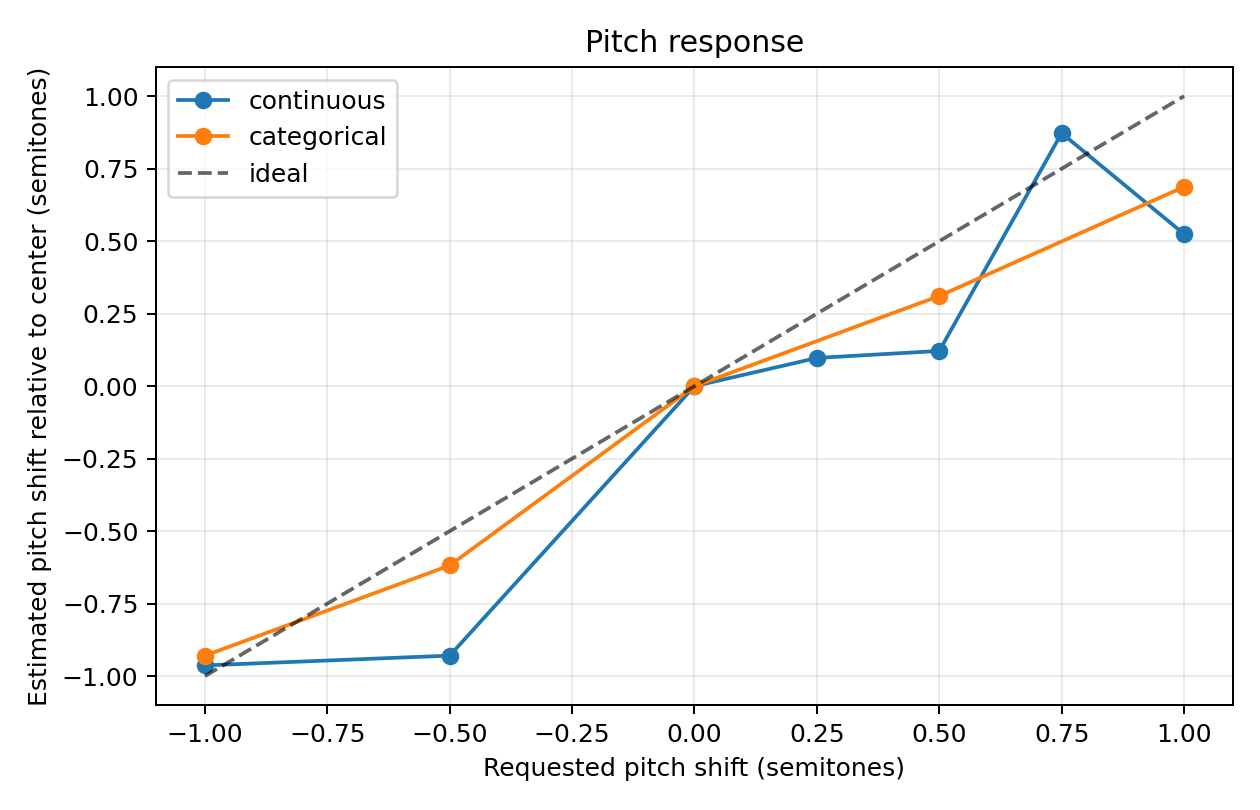
\includegraphics[width=\linewidth]{../../results/figures/pitch_response_curve.png}
  \caption{Pitch response curve for the main long run comparison. The figure summarizes how the estimated pitch shift follows the requested condition across the discrete sweep.}
  \label{fig:pitch_response}
\end{figure}

\begin{figure}[t]
  \centering
  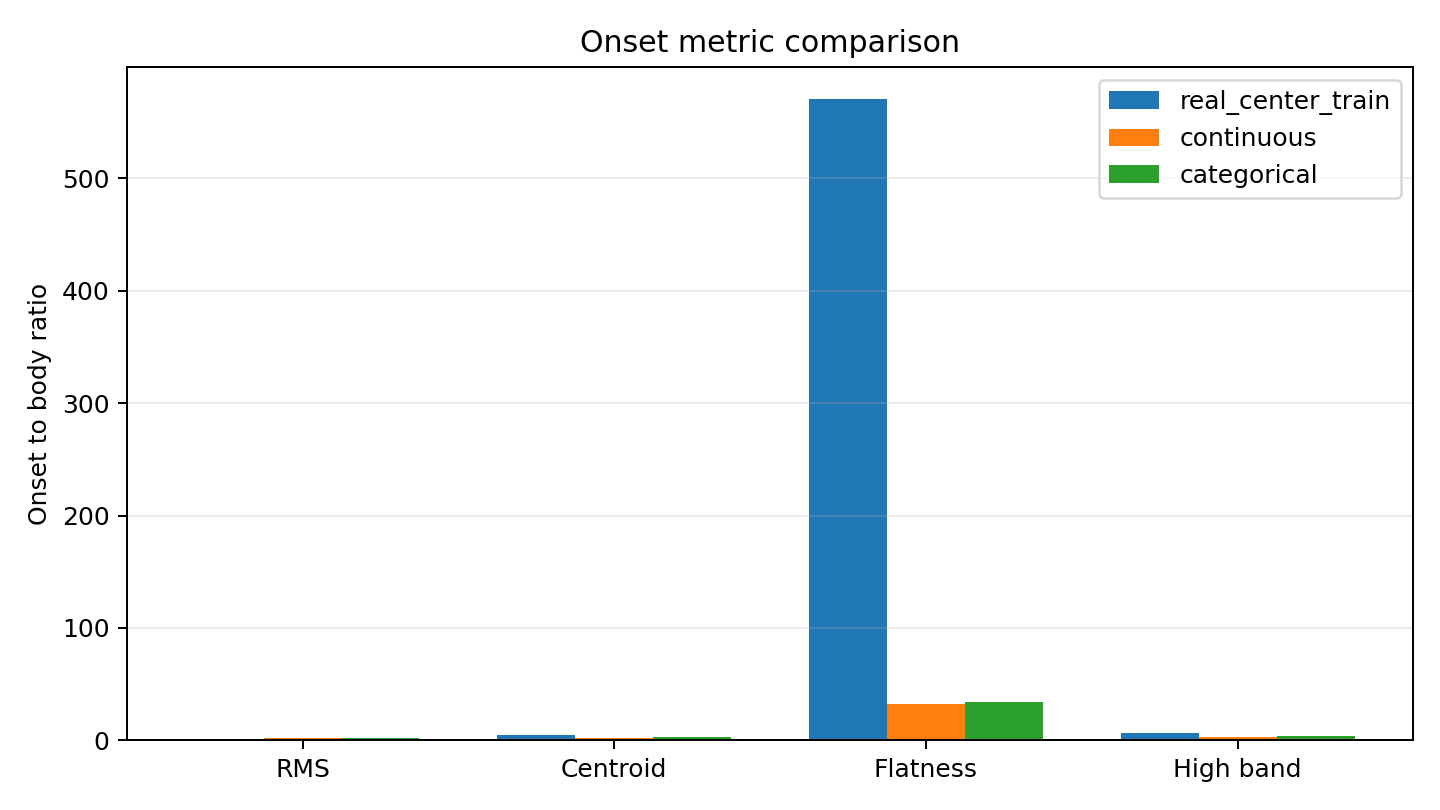
\includegraphics[width=\linewidth]{../../results/figures/onset_metric_comparison.png}
  \caption{Comparison of onset related objective metrics between the real training reference and the generated outputs. Lower ratios indicate a less exaggerated attack relative to the body of the sound.}
  \label{fig:onset_metrics}
\end{figure}

The main side by side comparison should use the Balanced profile. It is not the absolute best continuous configuration, but it keeps both models monotonic under the same decoding setup and therefore provides the cleanest shared reference for the paper, notebook, and oral demo. Under this profile, the continuous model reaches a discrete pitch MAE of \texttt{0.161} semitones, while the categorical model remains monotonic but with a higher error of \texttt{0.263} semitones.

The Cool profile is useful as a secondary ablation. It gives the continuous model its best discrete pitch MAE among the tested profiles and enables monotonic interpolation at both \texttt{+0.25} and \texttt{+0.75} semitones. However, the same decoding setup breaks the categorical model, which loses monotonicity and rises to \texttt{1.972} semitones of discrete pitch MAE.

The additional fine tuning stage lowered validation loss for both models, but only the continuous model improved in generation. The fine tuned continuous model reduced discrete pitch MAE from \texttt{0.264} to \texttt{0.169} semitones, while the fine tuned categorical model degraded from \texttt{0.138} to \texttt{1.733} semitones and lost monotonicity. This confirms that validation loss alone is not a sufficient proxy for controllability.

\section{Discussion}\label{sec:discussion}

Three conclusions emerge from the current experiments. First, the representation of the control parameter and the decoding policy interact strongly, so they should not be studied in isolation. Second, continuous conditioning benefits more from carefully tuned sampling and can support meaningful interpolation between seen pitch levels. Third, the categorical model can still be useful under balanced settings, but it is more sensitive to aggressive decoding changes in this setup than initially expected.

The onset artifact remains unresolved. Even in the best shared profile, the generated audio still shows an onset to body RMS ratio far above the real reference audio. This means that the pitch control comparison is already informative, but the synthesis quality itself still has room to improve.

\section{Limitations}\label{sec:limitations}

The source material is still melodic rather than purely textural, which may reduce how clearly conditioning behavior can be isolated. The compute budget also limited the number of long runs and prevented a broader hyperparameter search. Finally, the current draft would benefit from denser inline figure references and a broader listening based evaluation.

\section{Future Directions}\label{sec:future_directions}

Three follow up directions are especially natural. First, the same protocol could be repeated on a more textural source, such as a short trill based dataset, to reduce melodic confounds. Second, a second conditioning variable such as reverberation or density could be added to test whether representation effects remain stable in a multi parameter setting. Third, a lightweight listening study could complement the current objective metrics and clarify how numerical controllability aligns with perceived usefulness.

\section{AI Usage Statement}\label{sec:ai_usage}

AI assistance was used to help organize code, scripts, notebook structure, and paper drafting inside the project repository. All experimental decisions, code execution, result inspection, and final wording were reviewed by the author.

\section{Conclusion}\label{sec:conclusion}

This study suggests that continuous and categorical pitch conditioning should not be compared only through training loss or a single listening example. Under the fairest shared inference profile, both variants remain usable, but the continuous model reaches lower pitch error and better stability. Under a colder sampling profile, the continuous model also demonstrates clean interpolation, while the categorical model collapses. For the current project, the Balanced profile is therefore the main reference profile, and the Cool profile is the secondary profile used to illustrate the interpolation potential of the continuous representation.

\bibliographystyle{IEEEtran}
\bibliography{references}

\end{document}
